\chapter{Demodulation Challeneges}
While analyzing the different demodulation algorithms and trying to improve their performance there were a few phenomena that were observed. there are a few things that were problematic for software based demodulation. Some of these items are definitely challenges to any kind of demodulation, but while inspecting performance of the algorithms the following items gave us difficulty: DC Offset, White Noise, RF Characteristics, and emphasis.

\section{Challenge: DC Offset}
An audio signal can be characterized by a sine wave. In order to get different sounds the frequency of the sign wave is changed and in the context here the two important frequencies are 1200Hz and 2200Hz. Since an audio is a sine wave, the average value should be zero. The zero value is commonly referred to as the ground of the audio signal, and as the definition would imply the signal should spend the same amount of time above ground as it does below ground. As the performance of the zero crossing algorithm was investigated it was very evident that this was a challenge. If one assumes that the signal is centered about zero, and it is not, some of the logical decisions that are made will not hold true. More information on this later, for now take a look at the following figure and notice that the signal is not centered around zero.
\begin{figure}
  \centering
	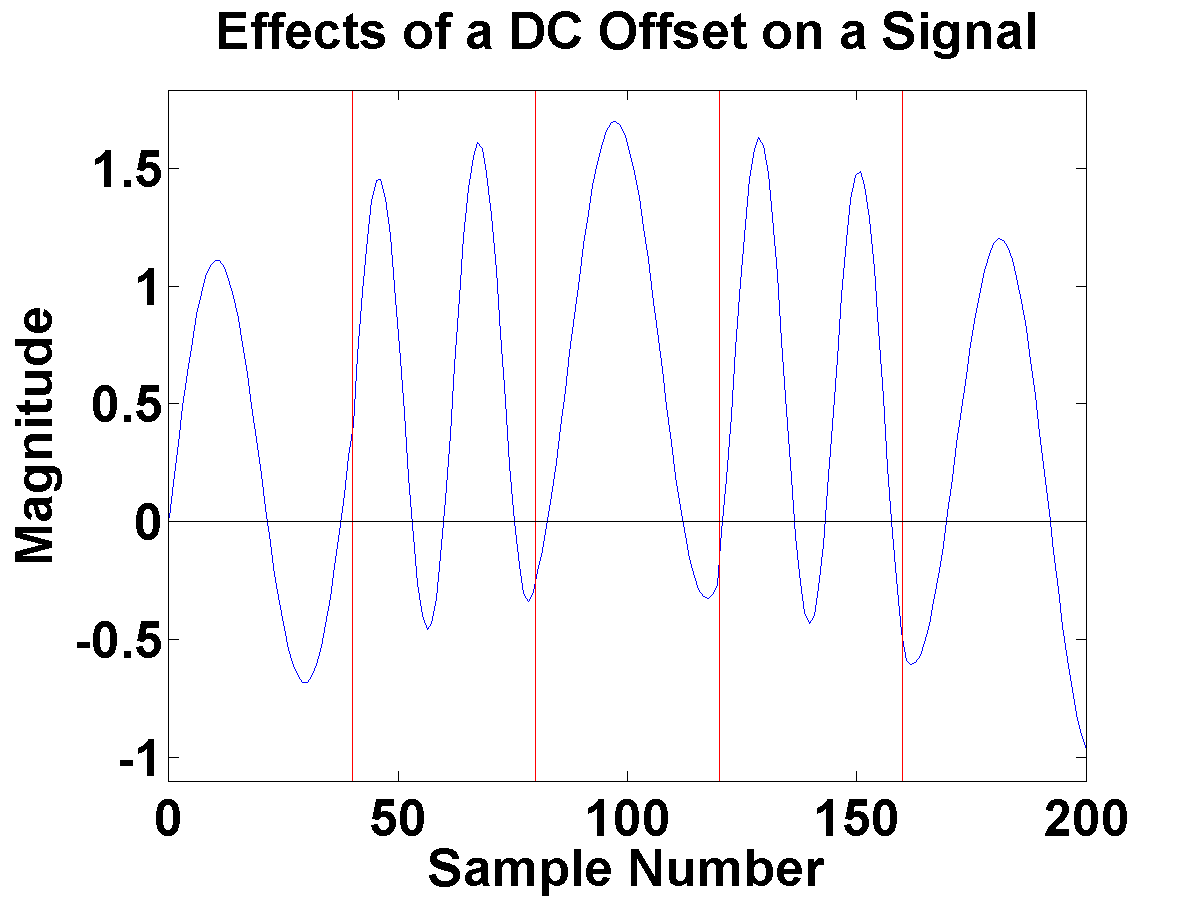
\includegraphics[width=0.75\linewidth]{images/EffectsofaDCOffsetonaSignal.png} 
	\caption{An Example Bell 202 signal with a DC offset Problem.}
\end{figure}

\section{Challenge: Noise And RF}
One other challenge was the fact that the digital stream in converted to an audio signal and then transmitted over RF. Since it is a FSK modulated signal that is decoded on the receiving end, ideally you would like the signal to come through as clean as possible. This is not the case for just the signals used in the specific application of APRS but with all wireless technologies. One cause is increased distance between the transmitter and receiver. An example that many are probably familiar with is as a client gets farther away from a wireless access point the bandwidth decreases. This happens because the signal strength drops off like 1 / distance cubed \cite{4Gon}. What was noticed when some of the algorithms were being debugged, was that the random noise that could be inflicted due to the nature of transmitting a wireless signal caused significant problems.

One such example of this is if the noise happened to also take on the form of a sine wave and the algorithm locked onto that frequency instead of the 1200Hz or 2200Hz signal that was wanted to be decoded. Alternatively, if the noise was just random and jostled the signal in the correct spot 1200Hz tones might look like 2200Hz (this ended up being fairly common) or vice versa. An example of what noise may look like on the original signal is in the figure below.
%\begin{figure}
%  \centering
%	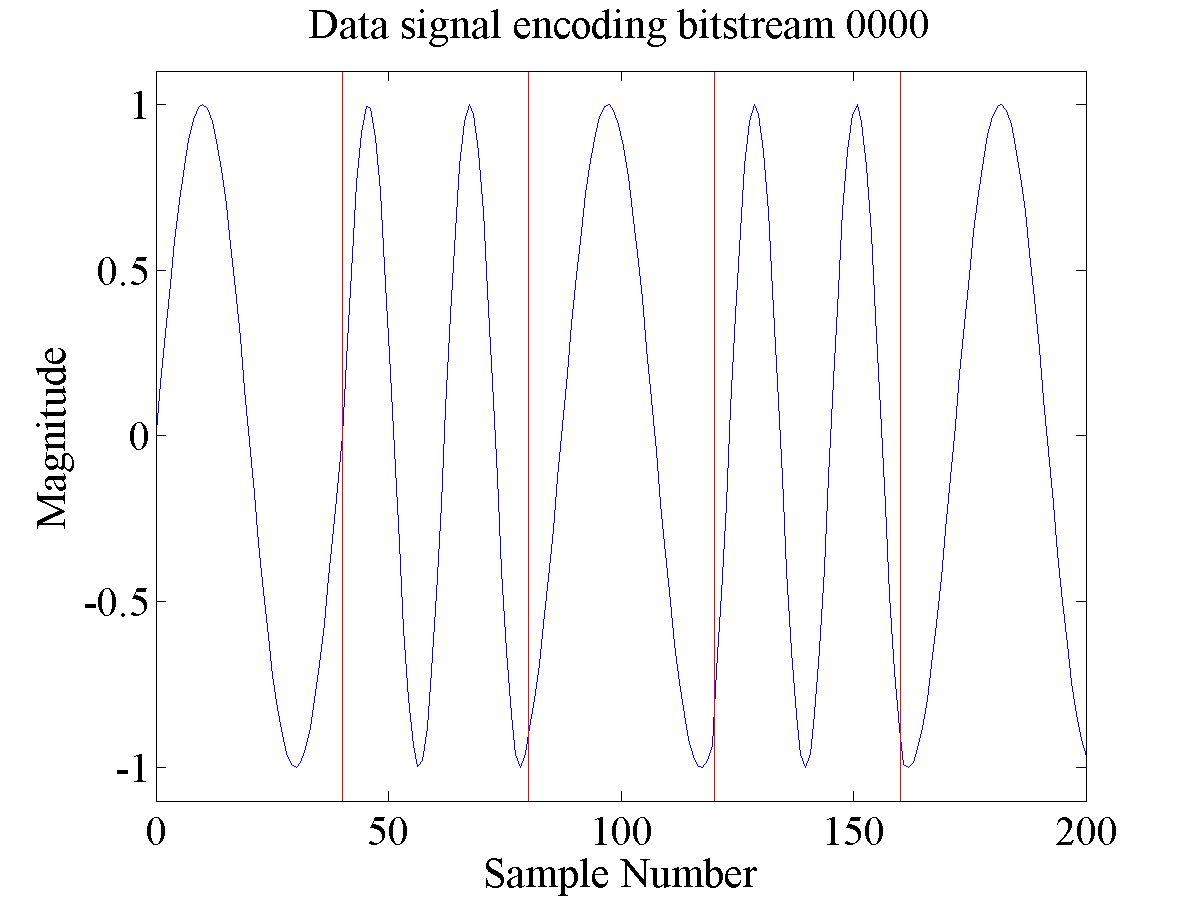
\includegraphics[width=0.75\linewidth]{images/Datasignalencodingbitstream0000.png} 
%	\caption{Example Bell 202 signal encoding the bit stream '0000'.}
%\end{figure}

%\section{Challenge: RF}

\section{Challenge: Emphasis}
The best has been saved for last, emphasis. Preemphasis is when the the higher audio tones in a Frequency Modulated (FM) signal are intentionally increased and deemphasis is when that process is revered on the receiving end to return the audio to a flat signal. Why do this? This process of emphasis is not necessary, but the effects are desirable since it increases the signal to noise ratio in the RF signal by having the higher audio tones preemphsized \cite{Gibilisco1994}. The effects of a non emphasized signal being deemphasized can be seen in the figure below.
\begin{figure}
  \centering
	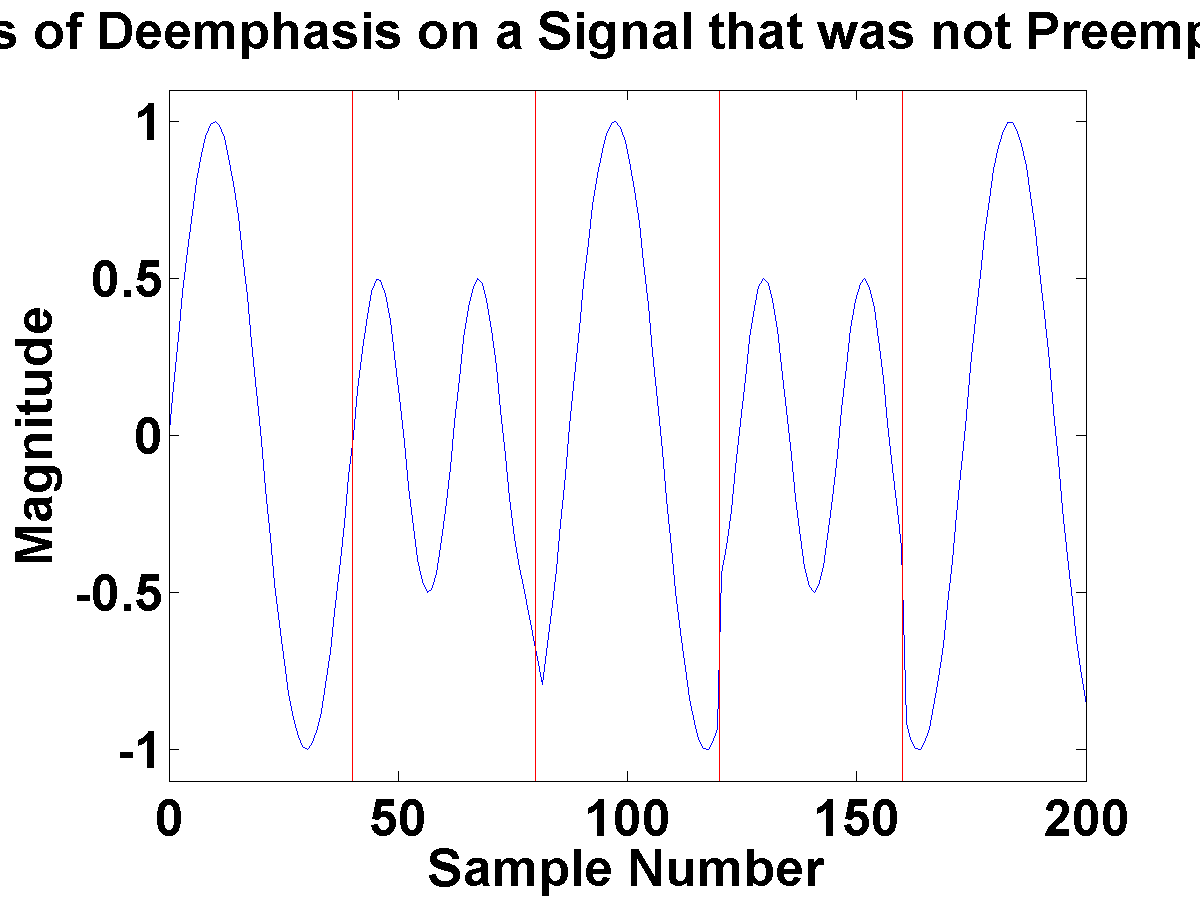
\includegraphics[width=0.75\linewidth]{images/EffectsofDeemphasisonaSignalthatwasnotpreemphasized.png} 
	\caption{An Example signal that was deemphasized, but not preemphasized.}
\end{figure}
